\documentclass[11pt,report]{article}

\usepackage[utf8x]{inputenc}
\usepackage[T1]{fontenc}
\usepackage[fleqn]{amsmath}
\usepackage{amssymb}
\usepackage{listings}
\usepackage{color}
\usepackage{makeidx}
\usepackage{blindtext}
\usepackage[table]{xcolor}% http://ctan.org/pkg/xcolor
\usepackage{float}
\usepackage{graphicx}
\usepackage{mathtools}
\usepackage{caption}
\usepackage{setspace}
\usepackage{subcaption}
\usepackage[hmargin=3cm,vmargin=3.5cm]{geometry}
\usepackage{indentfirst}
\definecolor{dkgreen}{rgb}{0,0.6,0}
\definecolor{gray}{rgb}{0.5,0.5,0.5}
\definecolor{mauve}{rgb}{0.58,0,0.82}
\usepackage{eurosym}
\usepackage{url}
\usepackage{tikz}
\usetikzlibrary{trees,arrows,calc}
\usetikzlibrary{shapes}

\lstset{frame=tb,
  language=SQL,
  aboveskip=3mm,
  belowskip=3mm,
  showstringspaces=false,
  columns=flexible,
  basicstyle={\small\ttfamily},
  numbers=none,
  numberstyle=\tiny\color{gray},
  keywordstyle=\color{blue},
  commentstyle=\color{dkgreen},
  stringstyle=\color{mauve},
  breaklines=true,
  breakatwhitespace=true
  tabsize=3
}


\usepackage{titlesec}
\titleformat{\section}{\hrule \large\bfseries}{\thesection}{1em}{}
\newcommand{\tab}{\hspace*{3em}}


\title{	Database Administration and Tuning \\ Mini-Project 2 - Report}
\author{
	Henrique Rocha - 68621 \\
	Ludijor Barros - 68626 \\
	Fábio Martins - 71073
}

\date{\today}
\begin{document}

	\maketitle
\section{Transaction Isolation Levels}
	{\color{gray}Present SQL Server T-SQL commands for accomplishing the following tasks:}
	\subsection{}
	{\color{gray}Create a database named NutrientsDB, containing one log file and three different data files, in three distinct filegroups (i.e., one data file in each filegroup). The log file should have an initial size of 25MB and a maximum size of 250MB. All data files should have an unlimited maximum size, except the one in the primary filegroup, which should have a maximum size of 1GB). The first data file on the first secondary filegroup should have an initial size of 100MB, and the remaining files should have an initial size of 50MB. All files should grow at a rate of 50\%, except for the data file in the primary filegroup, which should grow by 5MB, every time this is required.}

\begin{lstlisting}
CREATE DATABASE NutrientsDB ON 
PRIMARY (
	NAME = NutrientsDB,
	FILENAME = 'd:\data\NutrientsDB_01.mdf',
	SIZE = 50MB, MAXSIZE = 1GB, FILEGROWTH = 5MB ),
FILEGROUP NutrientsDB_02 (
	NAME = 'NutrientsDB_02', 
	FILENAME = 'd:\data\NutrientsDB_02.ndf', 
	SIZE = 100MB, MAXSIZE=UNLIMITED, FILEGROWTH = 50% ),
FILEGROUP NutrientsDB_03 (
	NAME = 'NutrientsDB_03', 
	FILENAME = 'd:\data\NutrientsDB_03.ndf', 
	SIZE = 50MB, MAXSIZE=UNLIMITED, FILEGROWTH = 50% )
LOG ON (
	NAME = 'NutrientsLog',
	FILENAME = 'd:\data\NutrientsLog.ldf',
	SIZE = 25MB, MAXSIZE = 250MB, FILEGROWTH = 50% );
\end{lstlisting}
%\lstinputlisting{mp1-Ex1-a.sql}

	\subsection{}
	{\color{gray}Create a table named Cheese in the NutrientsDB database. The table should have a numeric attribute named cheeseID, that identifies the individual records, an alphanumeric attribute named Type, and four other numeric attributes named Calories, Proteins, Carbohidrates, and Fat. The table should be partitioned so that all tuples where cheeseID is less or equal than 50 are physically stored in the primary filegroup, all tuples where the cheeseID is greater than 50, but less or equal than 100, are physically stored in the first secondary filegroup, and the remaining tuples are physically stored in the second secondary filegroup.}

\begin{lstlisting}
USE NutrientsDB;

CREATE PARTITION FUNCTION NutrientsPartitionFunction(NUMERIC)
AS RANGE LEFT FOR VALUES(50, 100);

CREATE PARTITION SCHEME NutrientsScheme
AS PARTITION NutrientsPartitionFunction
TO ([PRIMARY], NutrientsDB_02, NutrientsDB_03);

CREATE TABLE Cheese (
  cheeseID NUMERIC PRIMARY KEY,
  Type NVARCHAR(25),
  Calories NUMERIC,
  Proteins NUMERIC,
  Carbohidrates NUMERIC,
  Fat NUMERIC
) ON NutrientsScheme(cheeseID);
\end{lstlisting}

	\subsection{}
	{\color{gray}In the table named Cheese, the amount of calories is stored in an attribute named Calories, in Kcals per 100 grams. Create an index over the table with a search key corresponding to the calories in cals per 100 grams, including the amount of protein and fat as additional attributes that are not part of the search key. The index should be physically stored in the primary filegroup. Indicate also if the index is clustered or non-clustered, justifying.}

\begin{lstlisting}
USE NutrientsDB;
CREATE NONCLUSTERED INDEX Nutrients_Calories_IX
ON Cheese(Calories)
INCLUDE (Proteins, Fat)
ON [PRIMARY];
\end{lstlisting}




	O índice deve ser non-clustered, pois os valores presentes na coluna Calories não têm critério de ordenação.





\section{Concurrency Control}
\subsection{}

{	\color{gray}
Consider the following schedule for three concurrent transactions:
}
{
	\color{gray}
	\begin{table}[H]
\centering
{\color{gray}
	\begin{tabular}{l|l|l|l|}
	\cline{2-4}
		                    & T1       & T2       & T3       \\ \hline
	\multicolumn{1}{|l|}{1} & write(A) &          &          \\ \hline
	\multicolumn{1}{|l|}{2} &          &          & write(B) \\ \hline
	\multicolumn{1}{|l|}{3} &          & write(A) &          \\ \hline
	\multicolumn{1}{|l|}{4} & write(B) &          &          \\ \hline
	\multicolumn{1}{|l|}{5} &          & write(B) &          \\ \hline
	\end{tabular}
}
	\end{table}

}

\subsubsection{}
{\color{gray}Is the schedule allowed in Strict 2-Phase Locking? Justify.}
\begin{center}
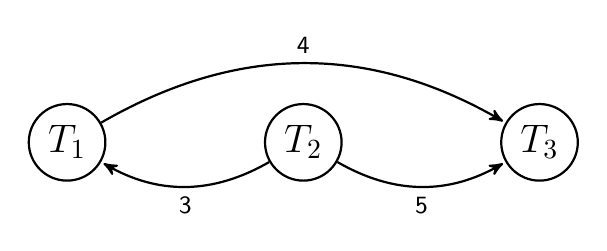
\begin{tikzpicture}[->,>=stealth',shorten >=1pt,auto,node distance=3cm,
  thick,main node/.style={circle,draw,font=\sffamily\Large\bfseries}]

  \node[main node] (1) {$T_1$};
  \node[main node] (2) [right of=1] {$T_2$};
  \node[main node] (3) [right of=2] {$T_3$};


  \path[every node/.style={font=\sffamily\small}]
    (2) edge [bend left] node[below] {3} (1)
    (2) edge [bend right] node[below] {5} (3)
    (1) edge [bend left] node {4} (3);
\end{tikzpicture}
\end{center}
	
	Yes, strict 2-Phase Locking allows only schedules whose precedence graph is acyclic, in this case the graph is acyclic.

\subsubsection{}

{\color{gray}Is the schedule allowed by the timestamp-based protocol? Justify.}

TS($T_1$)=1

TS($T_2$)=3

TS($T_3$)=2

\begin{table}[h]
\centering
\begin{tabular}{c|c|c|c|c|}
\cline{2-5}
                        & \multicolumn{2}{c|}{A} & \multicolumn{2}{c|}{B} \\ \hline
\multicolumn{1}{|c|}{t} & Rts(A)    & Wts(A)   & Rts(B)    & Wts(B)   \\ \hline
\multicolumn{1}{|c|}{1} & 0          & 1         & 0          & 0         \\ \hline
\multicolumn{1}{|c|}{2} & 0          & 1         & 0          & 2         \\ \hline
\multicolumn{1}{|c|}{3} & 0          & 3         & 0          & 2         \\ \hline
\multicolumn{1}{|c|}{4} &            &           &            &           \\ \hline
\multicolumn{1}{|c|}{5} &            &           &            &           \\ \hline
\end{tabular}
\end{table}

No, at $t=4$ transaction $T_1$ issues \textbf{write}(B), $[ TS(T_1)=1 ] < [ Wts(B) = 2 ]$, which means that $T_1$ is attempting to write an obsolete value of B, hence this write operation is rejected, $T_1$ is rolled back. 


\subsection{}
{\color{gray}Consider the following schedule for two concurrent transactions:}

\begin{table}[h]
\centering
{\color{gray}
\begin{tabular}{|c|c|c|}
\hline
  & T1        & T2        \\ \hline
1 & lock-S(A) &           \\ \hline
2 & read(A)   &           \\ \hline
3 & unlock(A) &           \\ \hline
4 &           & lock-X(B) \\ \hline
5 &           & write(B)  \\ \hline
6 &           & unlock(B) \\ \hline
7 & lock-S(B) &           \\ \hline
8 & read(B)   &           \\ \hline
9 & unlock(B) &           \\ \hline
\end{tabular}
}
\end{table}

\subsubsection{}
{\color{gray}Is the schedule allowed in Strict 2-Phase Locking? Justify.}

{\color{red}XXXXXXXXXXXXXXXXXXXXXXXXXXXXXXXXXXXXXXXXX}
\subsubsection{}
{\color{gray}Is the schedule allowed by the timestamp-based protocol? Justify.}

{\color{red}XXXXXXXXXXXXXXXXXXXXXXXXXXXXXXXXXXXXXXXXX}

\section{Recovery System}
	{\color{gray}Present SQL Server T-SQL commands for accomplishing the following tasks:}
	\subsection{}
	{\color{gray}Create a database named NutrientsDB, containing one log file and three different data files, in three distinct filegroups (i.e., one data file in each filegroup). The log file should have an initial size of 25MB and a maximum size of 250MB. All data files should have an unlimited maximum size, except the one in the primary filegroup, which should have a maximum size of 1GB). The first data file on the first secondary filegroup should have an initial size of 100MB, and the remaining files should have an initial size of 50MB. All files should grow at a rate of 50\%, except for the data file in the primary filegroup, which should grow by 5MB, every time this is required.}

\begin{lstlisting}
CREATE DATABASE NutrientsDB ON 
PRIMARY (
	NAME = NutrientsDB,
	FILENAME = 'd:\data\NutrientsDB_01.mdf',
	SIZE = 50MB, MAXSIZE = 1GB, FILEGROWTH = 5MB ),
FILEGROUP NutrientsDB_02 (
	NAME = 'NutrientsDB_02', 
	FILENAME = 'd:\data\NutrientsDB_02.ndf', 
	SIZE = 100MB, MAXSIZE=UNLIMITED, FILEGROWTH = 50% ),
FILEGROUP NutrientsDB_03 (
	NAME = 'NutrientsDB_03', 
	FILENAME = 'd:\data\NutrientsDB_03.ndf', 
	SIZE = 50MB, MAXSIZE=UNLIMITED, FILEGROWTH = 50% )
LOG ON (
	NAME = 'NutrientsLog',
	FILENAME = 'd:\data\NutrientsLog.ldf',
	SIZE = 25MB, MAXSIZE = 250MB, FILEGROWTH = 50% );
\end{lstlisting}

	\subsection{}
	{\color{gray}Create a table named Cheese in the NutrientsDB database. The table should have a numeric attribute named cheeseID, that identifies the individual records, an alphanumeric attribute named Type, and four other numeric attributes named Calories, Proteins, Carbohidrates, and Fat. The table should be partitioned so that all tuples where cheeseID is less or equal than 50 are physically stored in the primary filegroup, all tuples where the cheeseID is greater than 50, but less or equal than 100, are physically stored in the first secondary filegroup, and the remaining tuples are physically stored in the second secondary filegroup.}

	\subsection{}
	{\color{gray}In the table named Cheese, the amount of calories is stored in an attribute named Calories, in Kcals per 100 grams. Create an index over the table with a search key corresponding to the calories in cals per 100 grams, including the amount of protein and fat as additional attributes that are not part of the search key. The index should be physically stored in the primary filegroup. Indicate also if the index is clustered or non-clustered, justifying.}


\section{Schema and Index Tuning}
{\color{gray}Consider the following relational schema:}
	
	\textbf{\color{gray}\tab CheeseProvenance(\underline{cheese-name}, region-name)}

	\textbf{\color{gray}\tab Location(\underline{region-name}, climate-type)}

{\color{gray}The relation CheeseProvenance stores information about the region where each cheese type is produced, and the relation Location stores information about the the regions that produce cheese.}

{\color{gray}All tuples have fixed size. The relation CheeseProvenance takes 1000 blocks and the relation Location has 2300 blocks. Each page of CheeseProvenance contains 120 tuples and each page of Location contains 100 tuples.}

{\color{gray} Compute the number of I/Os performed by each of the following algorithms:}

	Data:

	\tab $b_r = 1000$ blocks

	\tab $b_s = 2300$ blocks

	\tab $|R|/b_r = 120$ tuples/block

	\tab $|S|/b_s = 100$ tuples/block


	\subsection{}
	{\color{gray} Selection on the Location relation where the filtering condition is climate-type = 'Dry', assuming there is an index on the table over the attribute climate-type.}
	\begin{equation}\sigma_{climate-type='Dry'}(Location)\end{equation}

	The selection operation is performed over an index, because this index isn't over the primary key, we can assume that it is non-clustering. Besides that, we are only testing for equality, that means that we must use algorithm 4 (A4) to retrieve multiple records (multiple locations).
	\begin{equation}Cost = (h_i + n) \end{equation}
		
	Where:

	\tab $n$ – number of records fetched (n=|S|, worst case)

	\tab $h_i$ – height of B+ tree

	With each I/O operation requiring a seek and a block transfer.


	% Database System Concepts, Pag 542
	

	\subsection{}
	{\color{gray} Block Nested Loop Join, with CheeseProvenance as the outer relation and the join condition is on region-name. Present the costs of the worst and best cases.}
	\begin{equation}CheeseProvenance \bowtie_{CheeseProvenance.region-name=Location.region-name} Location\end{equation}

	Worst case:
	\begin{equation}Cost = (b_r * b_s + b_r) $block transfers$\end{equation}
	%  (+ 2 * b_r $seeks$)
	Best case (if $b_r$ and $b_s$ fits in memory):
	\begin{equation}Cost = (b_r + b_s) $block transfers$\end{equation}
	% (+ 2 $seeks$)
	% Database System Concepts, Pag 551
	

	\subsection{}
	{\color{gray}Sort-Merge Join, assuming that only the relation Location is ordered on region-name, the relation CheeseProvenance is ordered on cheese-name and that you can have 3 pages in memory when sorting the relations.}
	\begin{equation}CheeseProvenance \bowtie_{CheeseProvenance.region-name=Location.region-name} Location\end{equation}

	Let:

	\tab $M = 3$ pages
	\begin{equation}Cost_{merge} = (b_r + b_s) \end{equation}
	\begin{equation}Cost_{sort} = 2b_s(\lceil log_{M-1}(b_s/M) \rceil+1) \end{equation}
	\begin{equation}Cost = Cost_{sort} + Cost_{merge} \end{equation}	



\section{Query Tuning}
{\color{gray} For each of the following queries, identify one possible reason why an optimizer might not find a good
execution plan. Rewrite the query so that a good plan is likely to be found. Any available indexes, or known
constraints, are listed before each query.}

{\color{gray}\subsection{} An index is available on the calories attribute:}

\begin{lstlisting}
SELECT type
FROM CHEESE
WHERE calories * 100 < 800
\end{lstlisting}

The optimizer might not find a good execution plan because the index over calories times 100 might not exist, a good solution is to divide 800 by 100.

\begin{lstlisting}
SELECT type
FROM CHEESE
WHERE calories < 8
\end{lstlisting}

It is important that the index is a b+ tree so the search for cheeses with calories lower then 8 is sequential after the first tree traversal.

{\color{gray}\subsection{} An index is available on the calories attribute:}

\begin{lstlisting}
SELECT type
FROM CHEESE
WHERE calories<90 AND calories>40
\end{lstlisting}

{\color{gray}\subsection{} A B+ Tree index is available on the calories attribute:}

\begin{lstlisting}
SELECT type
FROM CHEESE
WHERE calories=90 OR calories=40
\end{lstlisting}

{\color{gray}\subsection{} No index is available:}

\begin{lstlisting}
SELECT DISTINCT CheeseId, type
FROM CHEESE 
\end{lstlisting}

{\color{gray}\subsection{} No index is available:}

\begin{lstlisting}
SELECT AVG (proteins)
FROM CHEESE
GROUP BY producer
HAVING type = "Alverca"
\end{lstlisting}

	
\section{Database Tuning}
{\color{gray}Answer the following questions, on the subject of the invited talk given by engineer Wilson Lucas, that you had the opportunity to attend on the 24th of May 2015.}

	\subsection{}
	
{\color{gray}One of the tasks of a DBA is to assure the high availability of the Databases being managed. This can be done in several ways. However, independently of the technique used, there are always trade-offs that one must take into account when choosing how to implement it (or even if it is worth implementing). Name and explain one such trade-off.}

To guarantee data high availablity in a database, it's important to ensure that the information is ready to be accessed fastly and eficiently at any moment.

To ensure such availablity, there are multiple techniques that a database administrator can apply. One of those techniques consists on creating indexes over table columns. Creating indexes can increase a faster access to information. However, the space that an index occupies is considerable compared to the space that a table occupies. It is wise to create indexes only over the needed columns and not for every column, in order to minimize the impact of indexes on disk storage.

	\subsection{}

{\color{gray}In theory, once our database is fully optimized, it should not be necessary to change it any further. In practice, on a database that is being used in a functioning organization, this is not the case. Explain why.}

	In a functioning organization, the way that data is accessed may not be uniform, leading to access data through unsuitable indexes. Altough there are mechanisms to choose a good query plan, it may be slow due to inexistent indexes. The database administrator has the goal to understand what's the best way to access information and act to improve it. A good index today may be worse tomorrow. 

	Another factor to take in account, is that data creation and deletion tends to degrade the access to it, due to internal fragmentation. A good maintenance practice is to recreate indexes over time, so they can occupy less space and be accessed sequentially.

	There is also the necessity do backup databases in order to decrease or prevent data loss caused by a failure. The existence of a database administrator is essential in critical situations like this, as data loss could have great costs for an organization.
\end{document}
